%%%%%%%%%%%%%%%%%%%%%%%%%%%%%%%%%%%%%%%%%%%%%%%%%%%%%%%%%%%%%%%%%%%%%%%%%%%%%%%%
\section{Benchmarks}
\label{sec:benchmarking}
%%%%%%%%%%%%%%%%%%%%%%%%%%%%%%%%%%%%%%%%%%%%%%%%%%%%%%%%%%%%%%%%%%%%%%%%%%%%%%%%

In this section we present benchmarks for calculations of the low 
Mellin moments of PDFs and of the $x$-dependence of PDFs. We provide a systematic
comparison between lattice-QCD results and determinations from global fitting
calculations.
%
%%%%%%%%%%%%%%%%%%%%%%%%%%%%%%%%%%%%%%%%%%%%%%%%%%%%%%%%%%%%%%%%%%%%%%%%%%%%%%%%
\subsection{Benchmark criteria for lattice QCD}
To accurately assess the current state-of-the-art for lattice calculations, we
follow a procedure inspired by the review of low-energy mesons undertaken 
by the Flavor Lattice Averaging Group (FLAG) \cite{Aoki:2016frl}. For each
lattice calculation, we assess the status of each source of uncertainty outlined
in Sec.~\ref{Sec:IntroLQCD}. We use a rating system inspired by FLAG, awarding a
blue star (\bstar) for sources of uncertainty that are well-controlled or very conservatively
estimated, a blue circle (\bcirc) for sources of uncertainty that have been controlled or estimated to some extent,
and a red square (\rsquare) for uncertainties that have not met our criteria or for which no estimate is given.

We present our determination of the current, state-of-the-art
``world average'' for lattice-QCD results of the benchmark quantities. and 
provide both summary tables and overview comparison plots. Following FLAG, we include only those results that
are published in peer-reviewed journals or that have appeared as preprints. Where
recent results are a clear update of previously published work, we do not 
include the earlier results in the global average, but include them in the bibliography. Finally,
we remark that our criteria, and the corresponding ratings, are chosen not only
to provide as fair an assessment of the relative merits of various calculations as
possible, but to be aspirational. Where lattice-QCD results do meet these
standards, we hope that the lattice community will work towards improved calculations
and greater precision as part of a concerted and inter-disciplinary effort to better understand
nucleon structure.
%

Where the following criteria are not met, we award a red square (\rsquare).
\begin{itemize}
\item {\bfseries Discretisation effects and the continuum limit.} We assume that the lattice actions are
${\cal O}(a)$-improved, that is, that the discretization errors vanish quadratically with the lattice spacing. 
For unimproved actions an additional lattice spacing is required. We require that these
criteria are satisfied in each case for at least one pion mass below 300 MeV.
\begin{itemize}
\item[\bstar] At least three lattice spacings with at least two lattice spacings below 0.1 fm and
a range of lattice spacings that satisfies $[a_{\mathrm{max}}/a_{\mathrm{min}}]^2 \geq 2$.
\item[\bcirc] At least two lattice spacings with at least one point below 0.1 fm and a range of lattice spacings 
that satisfies $[a_{\mathrm{max}}/a_{\mathrm{min}}]^2 \geq 1.4$.
\end{itemize}
To receive a \bstar~or \bcirc~either a continuum extrapolation must be performed or the results must
demonstrate no significant discretisation effects over the appropriate range of lattice spacings.

\item {\bfseries Unphysical pion masses.} For the following criteria, we define a physical pion mass ensemble 
to be one with $M_\pi=135\pm 10$~MeV.
\begin{itemize}
\item[\bstar] One ensemble with a physical pion mass \emph{or} a chiral extrapolation with three or more pion masses,
with at least two pion masses below 250 MeV and at least one below 200~MeV.
\item[\bcirc] A chiral extrapolation with three or more pion mass, two of which are below 300~MeV.
\end{itemize}

\item {\bfseries Finite volume effects.} For calculations that use a mixed action approach, that is,
with different lattice actions for the valence and sea quarks, we apply the criteria for $M_\pi L$ to the valence quarks.
\begin{itemize}
\item[\bstar] Ensembles with $M_{\pi,\mathrm{min}}L\geq 4$, \emph{or} at least three volumes with spatial extent
$L>2.5$~fm.
\item[\bcirc] Ensembles with $M_{\pi,\mathrm{min}}L \geq 3.4$, \emph{or} at least two volumes with spatial extent
$L>2.5$~fm.
\end{itemize}

\item {\bfseries Excited state contamination.} The following criteria must be satisfied for every pion mass and lattice spacing.
\begin{itemize}
\item[\bstar] At least three source-sink  separations or a variational method to optimise the
operator derived from at least a $3\times 3$ correlator matrix. 
\item[\bcirc] Two source-sink separations at every pion mass and lattice spacing, or three or more source-sink separations at one pion mass
below 300~MeV. For the variational method, an optimised operator derived from a $2\times 2$ correlator matrix at every pion mass and
lattice spacing, or a $3\times 3$ correlator matrix for two pion masses below 300 MeV.
\end{itemize}

\item {\bfseries Renormalization.} 
\begin{itemize}
\item[\bstar] Nonperturbative renormalisation.
\item[\bcirc] Perturbative renormalisation.
\end{itemize}
For the axial coupling, $g_A$, we also award a \bstar~for calculations that use fermion actions for which $Z_A/Z_V=1$ or employ combinations of quantities for which the renormalisation is unity by construction.

\item {\bfseries Lattice-spacing determination.} For lattice-QCD calculations of nucleons, the lattice-spacing determination is generally 
sufficiently precise that it is a very small or negligible source
of systematic uncertainty. Therefore we do not include an assessment of the lattice-spacing
determination in our criteria.

\end{itemize}

%%%%%%%%%%%%%%%%%%%%%%%%%%%%%%%%%%%%%%%%%%%%%%%%%%%%%%%%%%%%%%%%%%%%%%%%%%%%%%%%
\subsection{Moments}

We provide a systematic comparison between existing
lattice-QCD results and PDF fitting calculations
for the lowest two moments of both unpolarized
and polarized PDFs. Current lattice calculations of higher moments are not sufficiently
controlled to allow meaningful comparison between lattice results and global fits.
With the exception of the axial coupling, $g_A$, there are no lattice calculations
for which all systematics have been fully explored and controlled. Therefore, 
for quantities other than $g_A$, we present a best-estimate band, rather than a global average. This band extends from the mean minus the error of the
smallest result to the mean plus the error of the largest, and includes all results
with two or more flavours of sea quarks, because current studies are not sufficiently
precise to distinguish between results with different numbers of sea quark flavours.
In three cases, $\langle x \rangle_{u,d,s}$, $\langle x \rangle_g$, $\langle 1 \rangle_{\Delta u,\Delta d}$, there is only one
lattice result available. For these quantities, our best-estimate band is given by this single result, but 
it should be noted that these results may underestimate some sources of uncertainty. We denote
these cases in Tables \ref{tab:LQCDunpol} and \ref{tab:LQCDpol0} with a superscript dagger.
In all benchmark tables, the moments are understood to be evaluated at a scale $\mu^2 = Q^2$, as outlined in Appendix 
\ref{sec:notation}. We provide complete listings of available results in Appendix \ref{sec:LQCDtables}.
%In all the cases, $\mu$ should be identified with the QCD
%factorization scale, the scale that separates long-distance from short-distance dynamics in perturbative
%factorization. Note that it is customary in PDF fits to assume
%$\mu=\mu_F=\mu_R$, though in principle the two scales
%could have different values.

%%%%%%%%%%%%%%%%%%%%%%%%%%%%%%%%%%%%%%%
\subsubsection{Unpolarized parton distributions}

\paragraph{First moments}
We summarise the current status of lattice-QCD calculations of the first moments of unpolarised PDFs
in Table \ref{tab:unpolLQCDstatus1}, including $\langle x\rangle_{u^+-d^+}$, $\langle x\rangle_{q^+}$ and
$\langle x\rangle_{g}$. We assess each calculation according 
to the criteria listed above. In the second column we indicate the number of sea quark flavours, $N_f$, and
in the third column we show whether the calculation has been published (P) or has appeared as a preprint (PreP).
We do not list results that have not been extrapolated to the physical pion mass, nor do we include 
quenched results in Table \ref{tab:unpolLQCDstatus1}. For completeness, we tabulate these results in Appendix 
\ref{sec:LQCDtables}.
\begin{table}
\renewcommand{\arraystretch}{1.2} 
\centering % See https://tex.stackexchange.com/questions/23650/when-should-we-use-begincenter-instead-of-centering
\makebox[\textwidth]{ % Centre table on page, even though it is a little wide
\begin{tabular}{lllccccccl}\\[1cm]
  Ref. & $N_f$ & Status & 
\hspace{0.15cm}\begin{rotate}{70}{discretisation}\end{rotate}\hspace{-0.15cm} &
\hspace{0.15cm}\begin{rotate}{70}{quark mass}\end{rotate}\hspace{-0.15cm} &
\hspace{0.15cm}\begin{rotate}{70}{finite volume}\end{rotate}\hspace{-0.15cm} &
\hspace{0.15cm}\begin{rotate}{70}{renormalisation}\end{rotate}\hspace{-0.15cm} &
\hspace{0.15cm}\begin{rotate}{70}{excited states}\end{rotate}\hspace{-0.15cm}&
 &  \\
  \hline%\hline
\multicolumn{10}{c}{$\langle x\rangle_{u^+-d^+}$}\\\hline
%\rowcolor{lightgray}
  LHPC 14 \cite{Green:2012ud} &
  2+1 & P & \rsquare & \bstar & \bstar & \bstar  &   \bstar & & 0.140(21)\\
%\rowcolor{lightgray}
  ETMC 17 \cite{Alexandrou:2017oeh} &
  2 & P &\rsquare  & \bstar &\rsquare  & \bstar  &   \bstar & $*$  & 0.194(9)(11)\\
%\rowcolor{lightgray}
  RQCD 14 \cite{Bali:2014gha} &
  2 &  P & \rsquare &\rsquare &\bcirc  & \bstar  &   \bstar & $**$ & 0.217(9) \\
\hline
\multicolumn{10}{c}{$\langle x\rangle_{u^+}$}\\\hline
%\rowcolor{lightgray}
  ETMC 17 \cite{Alexandrou:2017oeh} &
  2 & PreP &\rsquare  & \bstar &\rsquare  & \bstar  &   \bstar & $*\triangleright$ & $0.453(57)(48)$\\
%\rowcolor{lightgray}
  \hline
\multicolumn{10}{c}{$\langle x\rangle_{d^+}$}\\\hline
  ETMC 17 \cite{Alexandrou:2017oeh} &  2 & PreP &\rsquare  & \bstar &\rsquare  & \bstar  &   \bstar & $*\triangleright$ & $0.259(57)(47)$\\
  \hline
\multicolumn{10}{c}{$\langle x\rangle_{s^+}$}\\\hline
%\rowcolor{lightgray}
  ETMC 17 \cite{Alexandrou:2017oeh} &  2 & PreP &\rsquare  & \bstar &\rsquare  & \bstar  &   \bstar & $*\triangleright$ & $0.092(41)(0)$\\
  \hline
\multicolumn{10}{c}{ $\langle x\rangle_{g}$}\\\hline
%\rowcolor{lightgray}
  ETMC 17 \cite{Alexandrou:2017oeh} &
  2 & PreP &\rsquare  & \bstar &\rsquare  & \bcirc  &   \bstar & $*$ & 0.267(22)(27)\\
\hline
\end{tabular}
} % End makebox
\begin{minipage}{0.95\linewidth} % Align with left edge of table
{\footnotesize 
\begin{itemize}
\item[$*$] Study employing a single physical pion mass ensemble.
\item[$**$] Study employing a single ensemble with $m_\pi=150$~MeV.
\item[$\triangleright$] The mixing with $\langle x\rangle_{g}$ is computed
perturbatively and found to be small, so is neglected. 
\end{itemize}
}
\end{minipage}
\caption{Status of current lattice-QCD calculations of the first moments of unpolarised PDFs.}
\label{tab:unpolLQCDstatus1}
\end{table}

%%%%%%%%%%%%%%%%%%%%%%%%%%%%%%%%%%%%%%%%%%%%%%%%%%%%%%%%%%%%%
%%%%%%%%%%%%%%%%%%%%%%%%%%%%%%%%%%%%%%%%%%%%%%%%%%%%%%%%%%%%%
\begin{table}
\renewcommand{\arraystretch}{1.2} 
\centering
\begin{tabular}{cc}
\hline 
\rule[-4 ex]{0pt}{7 ex}  %% add some extra space
Moment & Benchmark \vspace*{-10pt}\\
\hline 
$\langle x \rangle_{u^+ -d^+}$ & \numrange{0.119}{0.226} \\
$\langle x \rangle_{u^+}$ & 0.453(75)$^\dagger$ \\
$\langle x \rangle_{d^+}$ & 0.259(74)$^\dagger$  \\
$\langle x \rangle_{s^+}$ & 0.092(41)$^\dagger$  \\
$\langle x\rangle_{g}$ & 0.267(35)$^\dagger$  \\
\hline 
\end{tabular}
\caption{Benchmark values for lattice calculations of the first moments of unpolarised PDFs. 
Results with a superscript $\dagger$ are from a single lattice calculation; these values may underestimate some sources of uncertainty.}
\label{tab:LQCDunpol}
\end{table}
%%%%%%%%%%%%%%%%%%%%%%%%%%%%%%%%%%%%%%%%%%%%%%%%%%%%%%%%%%%%%
%%%%%%%%%%%%%%%%%%%%%%%%%%%%%%%%%%%%%%%%%%%%%%%%%%%%%%%%%%%%%

\paragraph{Second moments}
In Appendix \ref{sec:LQCDtables}, we summarise the current status of lattice-QCD calculations of the second moment of 
the unpolarised valence quark PDFs, including $\langle x^2 \rangle_{u^-}$ and $\langle x^2\rangle_{u^--d^-}$. 
The study of these moments is not sufficiently mature to provide benchmark values and we only list the results for completeness.

%%%%%%%%%%%%%%%%%%%%%%%%%%%%%%%%%%%%%%%
\subsubsection{Polarized parton distributions}

\paragraph{Zeroth moments}

The zeroth moment of the helicity distribution is related to the axial charge of the 
nucleon, $g_A\equiv \langle 1\rangle_{\Delta u^+-\Delta d^+}$.
This quantity is of central importance to nucleon physics and
has long been considered an important benchmark for lattice calculations. Historically, 
lattice-QCD calculations of the axial charge have underestimated the experimental
value $g_A^{\mathrm{exp}} = 1.2723(23)$ \cite{Olive:2016xmw}, which is most precisely determined from cold 
neutron decays. Thus the axial charge has been the single most-studied moment in lattice QCD
and we provide a summary table of the current status of these calculations in Table \ref{tab:gAstatus}.
\begin{table}
\renewcommand{\arraystretch}{1.2} 
\centering
\begin{tabular}{lllccccccl}\\[1cm]
  Ref. & $N_f$ & Status & 
\hspace{0.15cm}\begin{rotate}{70}{discretisation}\end{rotate}\hspace{-0.15cm} &
\hspace{0.15cm}\begin{rotate}{70}{quark mass}\end{rotate}\hspace{-0.15cm} &
\hspace{0.15cm}\begin{rotate}{70}{finite volume}\end{rotate}\hspace{-0.15cm} &
\hspace{0.15cm}\begin{rotate}{70}{renormalisation}\end{rotate}\hspace{-0.15cm} &
\hspace{0.15cm}\begin{rotate}{70}{excited states}\end{rotate}\hspace{-0.15cm}&
 &  \\\hline%\hline
\multicolumn{10}{c}{$g_A\equiv \langle 1\rangle_{\Delta u^+-\Delta d^+}$}\\
  \hline
%\rowcolor{lightgray}
  CalLat 17 \cite{Berkowitz:2017gql} &
  2+1+1 & PreP & \rsquare  & \bstar  & \rsquare & \bstar &  \bstar& $\diamond$ & 1.278(21)(26) \\
%\rowcolor{lightgray}
  PNDME 16 \cite{Bhattacharya:2016zcn} &
  2+1+1 & P & \bcirc &\bstar  & \bcirc & \bstar  &   \bstar & & 1.195(33)(20)\\%\hline
  LHPC 14 \cite{Green:2012ud} &
  2+1 & P & \rsquare & \bstar & \bstar & \bstar  &   \bstar & & 0.97(8)\\%\hline
%\rowcolor{lightgray}
  Mainz 17 \cite{Capitani:2017qpc} &
  2 & PreP & \bstar & \bcirc & \bstar & \bstar  &   \bstar & & $1.278(68)({}^{+0}_{-0.087})$\\
%\rowcolor{lightgray}
  ETMC 17 \cite{Alexandrou:2017hac} &
  2 & PreP &\rsquare  & \bstar &\rsquare  & \bstar  &   \bstar & $*$ & 1.212(33)(22)\\
%\rowcolor{lightgray}
  RQCD 15 \cite{Bali:2014nma} &
  2 &  P & \bcirc &\bcirc  &\bcirc  & \bstar  &   \bcirc & $\ddag$& 1.280(44)(46) \\
  QCDSF 14 \cite{Horsley:2013ayv} &
  2 &  P & \bcirc &\bcirc  &\bcirc  & \bstar  &   \rsquare & $\ddag$& 1.29(5)(3) \\\hline%\hline
\end{tabular}
\begin{minipage}{0.94\linewidth}
{\footnotesize 
\begin{itemize}
\item[$*$] Study employing a single physical pion mass ensemble.
\item[$^\ddag$] $g_A$ is determined via the ratio $g_A/f_\pi$ employing the physical
value for $f_\pi$.
\item[$\diamond$] Approach inspired by the Feynman-Hellmann method is employed.
\end{itemize}
}
\end{minipage}
\caption{Status of current lattice-QCD calculations of the axial coupling, 
$g_A\equiv \langle 1\rangle_{\Delta u^+-\Delta d^+}$. Studies with three or more red squares are omitted from this table.}
\label{tab:gAstatus}
\end{table}

To provide benchmarks for the axial coupling, we use an approach based on the FLAG procedure. We distinguish between
calculations that use different numbers of sea quarks and exclude results that do not meet the criteria listed above. For 
$N_f = 2+1+1$, there is only a single calculation that satisfies these criteria \cite{Bhattacharya:2016zcn}. For $N_f = 2$,
we apply a weighted average of \cite{Capitani:2017qpc} and \cite{Bali:2014nma}, assuming correlations between the results and applying the procedure
of \cite{XXX}. Thus we obtain
\begin{equation}\label{eq:gAcriteria}
g_A^{N_f=2+1+1} = 1.195(33)(20)\,,\qquad \mathrm{and}\qquad g_A^{N_f=2+1+1} = 1.279(50).
\end{equation}

For the $N_f = 2+1+1$ result, there is only a single calculation, and this value may underestimate some sources of systematic uncertainty. To incorporate
information from the result of \cite{Berkowitz:2017gql}, which uses the same gauge configurations, we also carry out a simultaneous fit to the two
sets of data. We use a fit function of the form
\begin{equation}
g_A^{\mathrm{fit}} = c_0 + c_1a + c_2a^2 + c_3M_\pi^2 + c_4M_\pi^2 \exp(−M_\pi L) +c_5M_\pi^2 \exp\left(-\frac{M_\pi^2}{\Lambda_{\mathrm{QCD}}^2}\right).
\end{equation}
The coefficient $c_1$ captures ${\cal O}(a)$ effects
present in the valence quark action of \cite{Bhattacharya:2016zcn}, while \cite{Berkowitz:2017gql} has discretisation effects starting at ${\cal O}(a^2)$. The 
term proportional to $c_4$ captures the leading finite-volume effects and $c_3$ and $c_5$ represent chiral extrapolation terms. Modifications to this fit form,
including  setting $c_5 = 0$,
have negligible effect on the fit results, within extrapolation uncertainties, and the final result is in very good agreement with a simple weighted average
of the two calculations, assuming 100\% correlations, which is $g_A^{N_f=2+1+1,\mathrm{avg}} = 1.243(36)$. Based on this fit, we find a best-estimate band
of
\begin{equation}\label{eq:gAfit}
g_A^{N_f=2+1+1,\mathrm{fit}} = \numrange{1.22}{1.28}.
\end{equation}

We plot all lattice results for the axial coupling listed in Table \ref{} in Figure \ref{fig:gaLQCDstatus}. We show the world average experimental value as a vertical
black line. The light grey bands for $N_f = 2+1+1$ and $N_f=2$ represent the best-estimate results of Equation \eqref{eq:gAcriteria} and the dark grey band for
$N_f = 2+1+1$ is the fit band of Equation \eqref{eq:gAfit}. The open symbols are results that are not included in the best-estimate values.
%%%%%%%%%%%%%%%%%%%%%%%%%%%%%%%%%%%%%%%%%%%%%%%%%%%%%%%%%%%%%%%%%%%%%
\begin{figure}
\begin{center}
  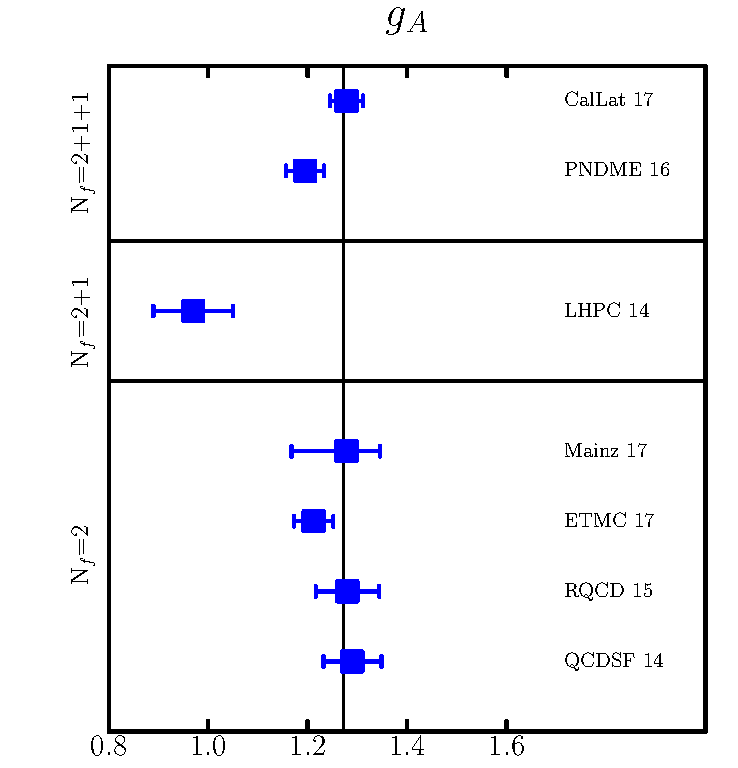
\includegraphics[scale=0.5]{plots/ga_summary.pdf}
  \caption{\small Summary of the current status of lattice-QCD calculations of the axial charge, $g_A\equiv \langle 1\rangle_{\Delta u^+-\Delta d^+}$.
  The vertical black line represents the current experimental world average $g_A^{\mathrm{exp}} = 1.2723(23)$ \cite{Olive:2016xmw}. The light grey bands for $N_f = 2+1+1$ and $N_f=2$ represent the best-estimate results of Equation \eqref{eq:gAcriteria} and the dark grey band for
$N_f = 2+1+1$ is the fit band of Equation \eqref{eq:gAfit}. The open symbols are results that are not included in the best-estimate values.
    \label{fig:gaLQCDstatus}
  }
\end{center}
\end{figure}
%%%%%%%%%%%%%%%%%%%%%%%%%%%%%%%%%%%%%%%%%%%%%%%%%%%%%%%%%%%%%%%%%%%%%%

In addition to the axial charge, we summarise the zeroth moments of the individual quark helicity distributions
in Table \ref{tab:polLQCDstatus0} and provide best-estimate benchmarks in Table \ref{tab:LQCDpol0}.
\begin{table}
\renewcommand{\arraystretch}{1.2} 
\centering
\makebox[\textwidth]{ % Centre table on page, even though it is a little wide
\begin{tabular}{lllccccccl}\\[1cm]
  Ref. & $N_f$ & Status & 
\hspace{0.15cm}\begin{rotate}{70}{discretisation}\end{rotate}\hspace{-0.15cm} &
\hspace{0.15cm}\begin{rotate}{70}{quark mass}\end{rotate}\hspace{-0.15cm} &
\hspace{0.15cm}\begin{rotate}{70}{finite volume}\end{rotate}\hspace{-0.15cm} &
\hspace{0.15cm}\begin{rotate}{70}{renormalisation}\end{rotate}\hspace{-0.15cm} &
\hspace{0.15cm}\begin{rotate}{70}{excited states}\end{rotate}\hspace{-0.15cm}&
 &  \\
  \hline%\hline
\multicolumn{10}{c}{$\langle 1\rangle_{\Delta u^+}$}\\\hline
%\rowcolor{lightgray}
  ETMC 17 \cite{Alexandrou:2017oeh} &
  2 & PreP &\rsquare  & \bstar &\rsquare  & \bstar  &   \bstar & $*$ & $0.830(26)(4)$\\
\hline
\multicolumn{10}{c}{$\langle 1\rangle_{\Delta d^+}$}\\\hline
%\rowcolor{lightgray}
  ETMC 17 \cite{Alexandrou:2017oeh} &
  2 & PreP &\rsquare  & \bstar &\rsquare  & \bstar  &   \bstar & $*$ & $-0.386(16)(6)$\\
\hline
\multicolumn{10}{c}{$\langle 1\rangle_{\Delta s^+}$}\\\hline
%\rowcolor{lightgray}
  $\chi$QCD 17 \cite{Gong:2015iir} &
  2+1 & P & \rsquare  & \bcirc & \bcirc  & \bstar  &  \bstar  & $\dagger$,$\triangleleft$ & -0.0403(44)(78)\\
%\rowcolor{lightgray}
  Engelhardt 12 \cite{Engelhardt:2012gd} &
  2+1 & P & \rsquare  & \rsquare & \bcirc  & \bstar  &  \bstar  & 
$\triangleleft$ & -0.031(17)\\
%\rowcolor{lightgray}
  ETMC 17 \cite{Alexandrou:2017oeh} &
  2 & PreP &\rsquare  & \bstar &\rsquare  & \bstar  &   \bstar & $*$ & -0.042(10)(2)\\
\hline
\end{tabular}
} % End makebox
\begin{minipage}{\linewidth}
{\footnotesize 
\begin{itemize}
\item[$*$] Study employing a single physical pion mass ensemble.
\item[$\dagger$] Partially quenched simulation with $m_\pi=330$~MeV. Criteria
applied to the valence quarks. 
\item[$\triangleleft$] Some parts of the renormalisation are estimated, see references for details.
\end{itemize}
}
\end{minipage}
\caption{Summary of the current status of lattice-QCD calculations of the zeroth moments of longitudinally polarised PDFs.}
\label{tab:polLQCDstatus0}
\end{table}

\begin{table}
\renewcommand{\arraystretch}{1.2} 
\centering
\begin{tabular}{cc}
\hline 
\rule[-4 ex]{0pt}{7 ex}  %% add some extra space
Moment & Benchmark value \vspace*{-10pt}\\
\hline 
$\langle 1 \rangle_{\Delta u}$ & 0.830(26)$^\dagger$ \\
$\langle 1 \rangle_{\Delta d}$ & -0.386(17)$^\dagger$  \\
$\langle 1 \rangle_{\Delta s}$ & \numrange{0.119}{0.226} \\
\hline 
\end{tabular}
\caption{Benchmark values for lattice calculations of the zeroth moments of polarised PDFs. Results with a superscript $\dagger$ are from a single lattice calculation; these values may underestimate some sources of uncertainty.}
\label{tab:LQCDpol0}
\end{table}



\paragraph{First moments} We summarise the status of lattice-QCD calculations of the
first moments of the longitudinally polarised PDF $\langle x \rangle_{\Delta u - \Delta d}$ in Table \ref{tab:polLQCDstatus1}. We
list the corresponding best-estimate benchmark in Table \ref{tab:LQCDpol1}.
\begin{table}
\renewcommand{\arraystretch}{1.2} 
\centering
\makebox[\textwidth]{ % Centre table on page, even though it is a little wide
\begin{tabular}{lllccccccl}\\[1cm]
  Ref. & $N_f$ & Status & 
\hspace{0.15cm}\begin{rotate}{70}{discretisation}\end{rotate}\hspace{-0.15cm} &
\hspace{0.15cm}\begin{rotate}{70}{quark mass}\end{rotate}\hspace{-0.15cm} &
\hspace{0.15cm}\begin{rotate}{70}{finite volume}\end{rotate}\hspace{-0.15cm} &
\hspace{0.15cm}\begin{rotate}{70}{renormalisation}\end{rotate}\hspace{-0.15cm} &
\hspace{0.15cm}\begin{rotate}{70}{excited states}\end{rotate}\hspace{-0.15cm}&
 &  \\
  \hline
\multicolumn{10}{c}{$\langle x\rangle_{\Delta u^--\Delta d^-}$}\\\hline
%\rowcolor{lightgray}
  RBC/UKQCD 10 \cite{Aoki:2010xg} &
  2+1 & P &\rsquare  & \rsquare &\bstar  & \bstar  &   \rsquare &  & 0.256(23),0.205(59)\\
%\rowcolor{lightgray}
  LHPC 10 \cite{Bratt:2010jn} &
  2+1 & P &\rsquare  & \rsquare &\bcirc  & \bcirc  &   \rsquare &  & 0.1972(55)\\
%\rowcolor{lightgray}
  ETMC 15 \cite{Abdel-Rehim:2015owa} &
  2 & P &\rsquare  & \bstar &\rsquare  & \bstar  &   \bstar & $*$ & 0.229(33)\\
\hline
\end{tabular}
} % End makebox
\begin{minipage}{\linewidth}
{\footnotesize 
\begin{itemize}
\item[$*$] Study employing a single physical pion mass ensemble.
\end{itemize}
}
\end{minipage}
\caption{Summary of the current status of lattice-QCD calculations of moments of longitudinally polarised PDFs.}
\label{tab:polLQCDstatus1}
\end{table}
%%%%%%%%%%%%%%%%%%%%%%%%%%%%%%%%%%%%%%%%%%%%%%%%%%%%%%%%%%%%%
%%%%%%%%%%%%%%%%%%%%%%%%%%%%%%%%%%%%%%%%%%%%%%%%%%%%%%%%%%%%%
\begin{table}
\renewcommand{\arraystretch}{1.2} 
\centering
\begin{tabular}{cc}
\hline 
\rule[-4 ex]{0pt}{7 ex}  %% add some extra space
Moment & Benchmark value \vspace*{-10pt}\\
\hline 
$\langle x \rangle_{\Delta u - \Delta d}$ & \numrange{0.146}{0.279}  \\
\hline 
\end{tabular}
\caption{Benchmark value for lattice calculations of the first moments of polarised PDFs.}
\label{tab:LQCDpol1}
\end{table}
%%%%%%%%%%%%%%%%%%%%%%%%%%%%%%%%%%%%%%%%%%%%%%%%%%%%%%%%%%%%%
%%%%%%%%%%%%%%%%%%%%%%%%%%%%%%%%%%%%%%%%%%%%%%%%%%%%%%%%%%%%%

\begin{comment}
%%%%%%%%%%%%%%%%%%%%%%%%%%%%%%%%%%%%%%%

\newpage
\textcolor{blue}{FIO: added sample tables copied from presentations; 
if the format is OK we can replace/update with the real benchmarks. }



%%%%%%%%%%%%%%%%%%%%%%%%%%%%%%%%%%%%%%%%%%%%%%%%%%%%%%%%%%%%%
%%%%%%%%%%%%%%%%%%%%%%%%%%%%%%%%%%%%%%%%%%%%%%%%%%%%%%%%%%%%%
\begin{table}[t]
\renewcommand{\arraystretch}{1.2} 
\centering
\begin{tabular}{@{}lccc@{}}
\hline 
\rule[-3 ex]{0pt}{7 ex}  %% add some extra space
$\left\langle x\right\rangle _{u}-\left\langle x\right\rangle _{d}$ 
   & Central Value & PDF error (\%) & Shift (\%) \\
\hline 
NNPDF3.0 & 0.102 & 2.4 & -\\
CT14 & 0.104 & 3.2 & +2.4\\
MMHT14 & 0.101 & 2.6 & -1.5\\
ABMP16 & 0.113 & 1.9 & +11\\
... &  &  & \\
\hline 
\end{tabular}
\caption{Benchmark for $\left\langle x\right\rangle _{u}-\left\langle x\right\rangle _{d}$
... at $Q=100$ GeV}
\end{table}
%%%%%%%%%%%%%%%%%%%%%%%%%%%%%%%%%%%%%%%%%%%%%%%%%%%%%%%%%%%%%
%%%%%%%%%%%%%%%%%%%%%%%%%%%%%%%%%%%%%%%%%%%%%%%%%%%%%%%%%%%%%

%%%%%%%%%%%%%%%%%%%%%%%%%%%%%%%%%%%%%%%%%%%%%%%%%%%%%%%%%%%%%
%%%%%%%%%%%%%%%%%%%%%%%%%%%%%%%%%%%%%%%%%%%%%%%%%%%%%%%%%%%%%
\begin{table}[t]
\renewcommand{\arraystretch}{1.2} 
\centering
\begin{tabular}{@{}lccc@{}}
\hline 
\rule[-3 ex]{0pt}{7 ex}  %% add some extra space
$\left\langle x\right\rangle _{\bar{u}}-\left\langle x\right\rangle _{\bar{d}}$ 
   & Central Value & PDF error (\%) & Shift (\%)\\
\hline 
NNPDF3.0 & -0.0038 & 51 & -\\
CT14 & -0.0055 & 25 & +43\\
MMHT14 & -0.0060 & 14 & +57\\
ABMP16 & -0.0059 & 11 & +54\\
... &  &  & \\
\hline 
\end{tabular}
\caption{Benchmark for $\left\langle x\right\rangle _{\bar{u}}-\left\langle x\right\rangle _{\bar{d}}$
... at $Q=5$ GeV}
\end{table}
%%%%%%%%%%%%%%%%%%%%%%%%%%%%%%%%%%%%%%%%%%%%%%%%%%%%%%%%%%%%%
%%%%%%%%%%%%%%%%%%%%%%%%%%%%%%%%%%%%%%%%%%%%%%%%%%%%%%%%%%%%%

%%%%%%%%%%%%%%%%%%%%%%%%%%%%%%%%%%%%%%%%%%%%%%%%%%%%%%%%%%%%%
%%%%%%%%%%%%%%%%%%%%%%%%%%%%%%%%%%%%%%%%%%%%%%%%%%%%%%%%%%%%%
\begin{table}[t]
\renewcommand{\arraystretch}{1.2} 
\centering
\begin{tabular}{@{}lccc@{}} 
\hline 
\rule[-3 ex]{0pt}{7 ex}  %% add some extra space
$\left\langle x\right\rangle _{s^{+}}$ 
   & Central Value & PDF error (\%) & Shift (\%) \\
\hline 
NNPDF3.0 & 0.46 & 6 & -\\
CT14 & 0.43 & 18 & -7\\
MMHT14 & 0.43 & 16 & -7\\
ABMP16 & 0.47 & 3 & +2\\
... &  &  & \\
\hline 
\end{tabular}

\caption{Benchmark for $\left\langle x\right\rangle _{s^{+}}$ ... at $Q=5$
GeV}
\end{table}
%%%%%%%%%%%%%%%%%%%%%%%%%%%%%%%%%%%%%%%%%%%%%%%%%%%%%%%%%%%%%
%%%%%%%%%%%%%%%%%%%%%%%%%%%%%%%%%%%%%%%%%%%%%%%%%%%%%%%%%%%%%

%%%%%%%%%%%%%%%%%%%%%%%%%%%%%%%%%%%%%%%%%%%%%%%%%%%%%%%%%%%%%
%%%%%%%%%%%%%%%%%%%%%%%%%%%%%%%%%%%%%%%%%%%%%%%%%%%%%%%%%%%%%
\begin{table}[t]
\renewcommand{\arraystretch}{1.2} 
\centering
\begin{tabular}{@{}lccc@{}}
\hline 
\rule[-3 ex]{0pt}{7 ex}  %% add some extra space
$\dfrac{\left\langle x\right\rangle _{s^{+}}}{\left\langle x\right\rangle _{\bar{u}}-\left\langle x\right\rangle _{\bar{d}}}$ 
   & Central Value & PDF error (\%) & Shift (\%)\\
\hline 
NNPDF3.0 & 0.64 & 8 & -\\
CT14 & 0.62 & 21 & -3\\
MMHT14 & 0.59 & 19 & -7\\
ABMP16 & 0.66 & 4 & 4\\
... &  &  & \\
\hline 
\end{tabular}
\caption{Benchmark for $\left\langle x\right\rangle _{s^{+}}/\left[\left\langle x\right\rangle _{\bar{u}}-\left\langle x\right\rangle _{\bar{d}}\right]$
... at $Q=5$ GeV}
\end{table}
%%%%%%%%%%%%%%%%%%%%%%%%%%%%%%%%%%%%%%%%%%%%%%%%%%%%%%%%%%%%%
%%%%%%%%%%%%%%%%%%%%%%%%%%%%%%%%%%%%%%%%%%%%%%%%%%%%%%%%%%%%%
\end{comment}
